\documentclass[1p]{elsarticle_modified}
%\bibliographystyle{elsarticle-num}

%\usepackage[colorlinks]{hyperref}
%\usepackage{abbrmath_seonhwa} %\Abb, \Ascr, \Acal ,\Abf, \Afrak
\usepackage{amsfonts}
\usepackage{amssymb}
\usepackage{amsmath}
\usepackage{amsthm}
\usepackage{scalefnt}
\usepackage{amsbsy}
\usepackage{kotex}
\usepackage{caption}
\usepackage{subfig}
\usepackage{color}
\usepackage{graphicx}
\usepackage{xcolor} %% white, black, red, green, blue, cyan, magenta, yellow
\usepackage{float}
\usepackage{setspace}
\usepackage{hyperref}

\usepackage{tikz}
\usetikzlibrary{arrows}

\usepackage{multirow}
\usepackage{array} % fixed length table
\usepackage{hhline}

%%%%%%%%%%%%%%%%%%%%%
\makeatletter
\renewcommand*\env@matrix[1][\arraystretch]{%
	\edef\arraystretch{#1}%
	\hskip -\arraycolsep
	\let\@ifnextchar\new@ifnextchar
	\array{*\c@MaxMatrixCols c}}
\makeatother %https://tex.stackexchange.com/questions/14071/how-can-i-increase-the-line-spacing-in-a-matrix
%%%%%%%%%%%%%%%

\usepackage[normalem]{ulem}

\newcommand{\msout}[1]{\ifmmode\text{\sout{\ensuremath{#1}}}\else\sout{#1}\fi}
%SOURCE: \msout is \stkout macro in https://tex.stackexchange.com/questions/20609/strikeout-in-math-mode

\newcommand{\cancel}[1]{
	\ifmmode
	{\color{red}\msout{#1}}
	\else
	{\color{red}\sout{#1}}
	\fi
}

\newcommand{\add}[1]{
	{\color{blue}\uwave{#1}}
}

\newcommand{\replace}[2]{
	\ifmmode
	{\color{red}\msout{#1}}{\color{blue}\uwave{#2}}
	\else
	{\color{red}\sout{#1}}{\color{blue}\uwave{#2}}
	\fi
}

\newcommand{\Sol}{\mathcal{S}} %segment
\newcommand{\D}{D} %diagram
\newcommand{\A}{\mathcal{A}} %arc


%%%%%%%%%%%%%%%%%%%%%%%%%%%%%5 test

\def\sl{\operatorname{\textup{SL}}(2,\Cbb)}
\def\psl{\operatorname{\textup{PSL}}(2,\Cbb)}
\def\quan{\mkern 1mu \triangleright \mkern 1mu}

\theoremstyle{definition}
\newtheorem{thm}{Theorem}[section]
\newtheorem{prop}[thm]{Proposition}
\newtheorem{lem}[thm]{Lemma}
\newtheorem{ques}[thm]{Question}
\newtheorem{cor}[thm]{Corollary}
\newtheorem{defn}[thm]{Definition}
\newtheorem{exam}[thm]{Example}
\newtheorem{rmk}[thm]{Remark}
\newtheorem{alg}[thm]{Algorithm}

\newcommand{\I}{\sqrt{-1}}
\begin{document}

%\begin{frontmatter}
%
%\title{Boundary parabolic representations of knots up to 8 crossings}
%
%%% Group authors per affiliation:
%\author{Yunhi Cho} 
%\address{Department of Mathematics, University of Seoul, Seoul, Korea}
%\ead{yhcho@uos.ac.kr}
%
%
%\author{Seonhwa Kim} %\fnref{s_kim}}
%\address{Center for Geometry and Physics, Institute for Basic Science, Pohang, 37673, Korea}
%\ead{ryeona17@ibs.re.kr}
%
%\author{Hyuk Kim}
%\address{Department of Mathematical Sciences, Seoul National University, Seoul 08826, Korea}
%\ead{hyukkim@snu.ac.kr}
%
%\author{Seokbeom Yoon}
%\address{Department of Mathematical Sciences, Seoul National University, Seoul, 08826,  Korea}
%\ead{sbyoon15@snu.ac.kr}
%
%\begin{abstract}
%We find all boundary parabolic representation of knots up to 8 crossings.
%
%\end{abstract}
%\begin{keyword}
%    \MSC[2010] 57M25 
%\end{keyword}
%
%\end{frontmatter}

%\linenumbers
%\tableofcontents
%
\newcommand\colored[1]{\textcolor{white}{\rule[-0.35ex]{0.8em}{1.4ex}}\kern-0.8em\color{red} #1}%
%\newcommand\colored[1]{\textcolor{white}{ #1}\kern-2.17ex	\textcolor{white}{ #1}\kern-1.81ex	\textcolor{white}{ #1}\kern-2.15ex\color{red}#1	}

{\Large $\underline{11n_{71}~(K11n_{71})}$}

\setlength{\tabcolsep}{10pt}
\renewcommand{\arraystretch}{1.6}
\vspace{1cm}\begin{tabular}{m{100pt}>{\centering\arraybackslash}m{274pt}}
\multirow{5}{120pt}{
	\centering
	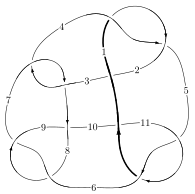
\includegraphics[width=112pt]{../../../GIT/diagram.site/Diagrams/png/687_11n_71.png}\\
\ \ \ A knot diagram\footnotemark}&
\allowdisplaybreaks
\textbf{Linearized knot diagam} \\
\cline{2-2}
 &
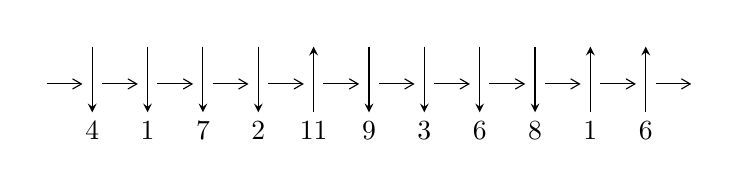
\begin{tikzpicture}[x=20pt, y=17pt]
	% nodes
	\node (C0) at (0, 0) {};
	\node (C1) at (1, 0) {};
	\node (C1U) at (1, +1) {};
	\node (C1D) at (1, -1) {4};

	\node (C2) at (2, 0) {};
	\node (C2U) at (2, +1) {};
	\node (C2D) at (2, -1) {1};

	\node (C3) at (3, 0) {};
	\node (C3U) at (3, +1) {};
	\node (C3D) at (3, -1) {7};

	\node (C4) at (4, 0) {};
	\node (C4U) at (4, +1) {};
	\node (C4D) at (4, -1) {2};

	\node (C5) at (5, 0) {};
	\node (C5U) at (5, +1) {};
	\node (C5D) at (5, -1) {11};

	\node (C6) at (6, 0) {};
	\node (C6U) at (6, +1) {};
	\node (C6D) at (6, -1) {9};

	\node (C7) at (7, 0) {};
	\node (C7U) at (7, +1) {};
	\node (C7D) at (7, -1) {3};

	\node (C8) at (8, 0) {};
	\node (C8U) at (8, +1) {};
	\node (C8D) at (8, -1) {6};

	\node (C9) at (9, 0) {};
	\node (C9U) at (9, +1) {};
	\node (C9D) at (9, -1) {8};

	\node (C10) at (10, 0) {};
	\node (C10U) at (10, +1) {};
	\node (C10D) at (10, -1) {1};

	\node (C11) at (11, 0) {};
	\node (C11U) at (11, +1) {};
	\node (C11D) at (11, -1) {6};
	\node (C12) at (12, 0) {};

	% arrows
	\draw[->,>={angle 60}]
	(C0) edge (C1) (C1) edge (C2) (C2) edge (C3) (C3) edge (C4) (C4) edge (C5) (C5) edge (C6) (C6) edge (C7) (C7) edge (C8) (C8) edge (C9) (C9) edge (C10) (C10) edge (C11) (C11) edge (C12) ;	\draw[->,>=stealth]
	(C1U) edge (C1D) (C2U) edge (C2D) (C3U) edge (C3D) (C4U) edge (C4D) (C5D) edge (C5U) (C6U) edge (C6D) (C7U) edge (C7D) (C8U) edge (C8D) (C9U) edge (C9D) (C10D) edge (C10U) (C11D) edge (C11U) ;
	\end{tikzpicture} \\
\hhline{~~} \\& 
\textbf{Solving Sequence} \\ \cline{2-2} 
 &
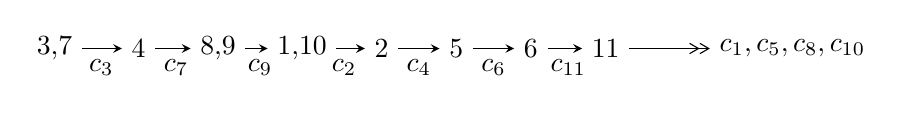
\begin{tikzpicture}[x=27pt, y=7pt]
	% node
	\node (A0) at (-1/8, 0) {3,7};
	\node (A1) at (1, 0) {4};
	\node (A2) at (33/16, 0) {8,9};
	\node (A3) at (51/16, 0) {1,10};
	\node (A4) at (17/4, 0) {2};
	\node (A5) at (21/4, 0) {5};
	\node (A6) at (25/4, 0) {6};
	\node (A7) at (29/4, 0) {11};
	\node (C1) at (1/2, -1) {$c_{3}$};
	\node (C2) at (3/2, -1) {$c_{7}$};
	\node (C3) at (21/8, -1) {$c_{9}$};
	\node (C4) at (15/4, -1) {$c_{2}$};
	\node (C5) at (19/4, -1) {$c_{4}$};
	\node (C6) at (23/4, -1) {$c_{6}$};
	\node (C7) at (27/4, -1) {$c_{11}$};
	\node (A8) at (39/4, 0) {$c_{1},c_{5},c_{8},c_{10}$};

	% edge
	\draw[->,>=stealth]	
	(A0) edge (A1) (A1) edge (A2) (A2) edge (A3) (A3) edge (A4) (A4) edge (A5) (A5) edge (A6) (A6) edge (A7) ;
	\draw[->>,>={angle 60}]	
	(A7) edge (A8);
\end{tikzpicture} \\ 

\end{tabular} \\

\footnotetext{
The image of knot diagram is generated by the software ``\textbf{Draw programme}" developed by Andrew Bartholomew(\url{http://www.layer8.co.uk/maths/draw/index.htm\#Running-draw}), where we modified some parts for our purpose(\url{https://github.com/CATsTAILs/LinksPainter}).
}\phantom \\ \newline 
\centering \textbf{Ideals for irreducible components\footnotemark of $X_{\text{par}}$} 
 
\begin{align*}
I^u_{1}&=\langle 
481 u^{12}-3744 u^{11}+\cdots+245268 d-61940,\;-4057 u^{12}-5862 u^{11}+\cdots+163512 c-19528,\\
\phantom{I^u_{1}}&\phantom{= \langle  }-664 u^{12}-4959 u^{11}+\cdots+122634 b+22418,\;15485 u^{12}+31932 u^{11}+\cdots+490536 a-416896,\\
\phantom{I^u_{1}}&\phantom{= \langle  }u^{13}+2 u^{12}+5 u^{11}+6 u^{10}+6 u^9+6 u^8- u^7-4 u^6-10 u^5-12 u^4+24 u^3-4 u^2+8\rangle \\
I^u_{2}&=\langle 
- u^3+a u+2 u^2+d-4 u+3,\;2 u^4 a-4 u^3 a- u^4+8 u^2 a+3 u^3-6 a u-6 u^2+2 c+2 a+7 u-4,\\
\phantom{I^u_{2}}&\phantom{= \langle  }- u^4 a+2 u^3 a-5 u^2 a+3 a u+u^2+b-2 a- u+2,\\
\phantom{I^u_{2}}&\phantom{= \langle  }3 u^4 a-9 u^3 a- u^4+16 u^2 a+3 u^3+2 a^2-17 a u-6 u^2+4 a+7 u-2,\;u^5-3 u^4+6 u^3-7 u^2+4 u-2\rangle \\
I^u_{3}&=\langle 
u^2+d,\;- u^2+c-1,\;2 a u- u^2+b+a- u,\;4 u^2 a+a^2+a u-3 u^2+6 a- u-5,\;u^3+u^2+2 u+1\rangle \\
I^u_{4}&=\langle 
u^2 c+c u- u^2+d+2 c- u-1,\;u^2 c+c^2- u^2+c-1,\;b- u,\;a+u,\;u^3+u^2+2 u+1\rangle \\
I^u_{5}&=\langle 
u^2+d,\;- u^2+c-1,\;b- u,\;a+u,\;u^3+u^2+2 u+1\rangle \\
\\
I^v_{1}&=\langle 
a,\;d+1,\;c- a+1,\;b+1,\;v+1\rangle \\
I^v_{2}&=\langle 
a,\;d,\;c-1,\;b+1,\;v-1\rangle \\
I^v_{3}&=\langle 
c,\;d-1,\;b,\;a-1,\;v-1\rangle \\
I^v_{4}&=\langle 
a,\;d a+c- v-1,\;d v-1,\;c v- v^2+a- v,\;b+1\rangle \\
\end{align*}
\raggedright * 8 irreducible components of $\dim_{\mathbb{C}}=0$, with total 41 representations.\\
\raggedright * 1 irreducible components of $\dim_{\mathbb{C}}=1$ \\
\footnotetext{All coefficients of polynomials are rational numbers. But the coefficients are sometimes approximated in decimal forms when there is not enough margin.}
\newpage
\renewcommand{\arraystretch}{1}
\centering \section*{I. $I^u_{1}= \langle 481 u^{12}-3744 u^{11}+\cdots+2.45\times10^{5} d-6.19\times10^{4},\;-4057 u^{12}-5862 u^{11}+\cdots+1.64\times10^{5} c-1.95\times10^{4},\;-664 u^{12}-4959 u^{11}+\cdots+1.23\times10^{5} b+2.24\times10^{4},\;1.55\times10^{4} u^{12}+3.19\times10^{4} u^{11}+\cdots+4.91\times10^{5} a-4.17\times10^{5},\;u^{13}+2 u^{12}+\cdots-4 u^2+8 \rangle$}
\flushleft \textbf{(i) Arc colorings}\\
\begin{tabular}{m{7pt} m{180pt} m{7pt} m{180pt} }
\flushright $a_{3}=$&$\begin{pmatrix}1\\0\end{pmatrix}$ \\
\flushright $a_{7}=$&$\begin{pmatrix}0\\u\end{pmatrix}$ \\
\flushright $a_{4}=$&$\begin{pmatrix}1\\u^2\end{pmatrix}$ \\
\flushright $a_{8}=$&$\begin{pmatrix}- u\\u\end{pmatrix}$ \\
\flushright $a_{9}=$&$\begin{pmatrix}0.0248116 u^{12}+0.0358506 u^{11}+\cdots-1.16261 u+0.119429\\-0.00196112 u^{12}+0.0152649 u^{11}+\cdots+0.849879 u+0.252540\end{pmatrix}$ \\
\flushright $a_{1}=$&$\begin{pmatrix}-0.0315675 u^{12}-0.0650961 u^{11}+\cdots-0.166977 u+0.849879\\0.00541449 u^{12}+0.0404374 u^{11}+\cdots+0.371969 u-0.182804\end{pmatrix}$ \\
\flushright $a_{10}=$&$\begin{pmatrix}-0.00479679 u^{12}-0.0550051 u^{11}+\cdots-0.979802 u+0.162744\\0.0276473 u^{12}+0.106121 u^{11}+\cdots+0.667074 u+0.209224\end{pmatrix}$ \\
\flushright $a_{2}=$&$\begin{pmatrix}-0.0177948 u^{12}-0.0521797 u^{11}+\cdots-0.286405 u+1.04837\\0.00289479 u^{12}+0.0135036 u^{11}+\cdots+0.261787 u-0.0657730\end{pmatrix}$ \\
\flushright $a_{5}=$&$\begin{pmatrix}-0.0261530 u^{12}-0.0246587 u^{11}+\cdots+0.204992 u+0.667074\\0.0454115 u^{12}+0.0564362 u^{11}+\cdots-0.162744 u-0.0383743\end{pmatrix}$ \\
\flushright $a_{6}=$&$\begin{pmatrix}-0.0228505 u^{12}-0.0511155 u^{11}+\cdots+0.312727 u-0.371969\\-0.00196112 u^{12}+0.0152649 u^{11}+\cdots+0.849879 u+0.252540\end{pmatrix}$ \\
\flushright $a_{11}=$&$\begin{pmatrix}-0.00615449 u^{12}-0.0166593 u^{11}+\cdots-0.562364 u+0.739289\\0.0254497 u^{12}+0.0984515 u^{11}+\cdots+0.788525 u+0.0840387\end{pmatrix}$\\ \flushright $a_{11}=$&$\begin{pmatrix}-0.00615449 u^{12}-0.0166593 u^{11}+\cdots-0.562364 u+0.739289\\0.0254497 u^{12}+0.0984515 u^{11}+\cdots+0.788525 u+0.0840387\end{pmatrix}$\\&\end{tabular}
\flushleft \textbf{(ii) Obstruction class $= -1$}\\~\\
\flushleft \textbf{(iii) Cusp Shapes $= -\frac{3739}{13626} u^{12}-\frac{4675}{13626} u^{11}-\frac{4243}{4542} u^{10}-\frac{6761}{13626} u^9-\frac{812}{6813} u^8-\frac{59}{757} u^7+\frac{14825}{13626} u^6-\frac{1951}{13626} u^5-\frac{811}{757} u^4-\frac{10702}{6813} u^3-\frac{80432}{6813} u^2+\frac{22922}{6813} u-\frac{4756}{2271}$}\\~\\
\newpage\renewcommand{\arraystretch}{1}
\flushleft \textbf{(iv) u-Polynomials at the component}\newline \\
\begin{tabular}{m{50pt}|m{274pt}}
Crossings & \hspace{64pt}u-Polynomials at each crossing \\
\hline $$\begin{aligned}c_{1},c_{4},c_{6}\\c_{8}\end{aligned}$$&$\begin{aligned}
&u^{13}-2 u^{12}+4 u^{10}-8 u^8+7 u^7+7 u^6-8 u^5-3 u^4+9 u^3+u^2- u+1
\end{aligned}$\\
\hline $$\begin{aligned}c_{2},c_{9}\end{aligned}$$&$\begin{aligned}
&u^{13}+4 u^{12}+\cdots- u+1
\end{aligned}$\\
\hline $$\begin{aligned}c_{3},c_{7}\end{aligned}$$&$\begin{aligned}
&u^{13}+2 u^{12}+\cdots-4 u^2+8
\end{aligned}$\\
\hline $$\begin{aligned}c_{5},c_{11}\end{aligned}$$&$\begin{aligned}
&u^{13}+2 u^{12}+\cdots+8 u+4
\end{aligned}$\\
\hline $$\begin{aligned}c_{10}\end{aligned}$$&$\begin{aligned}
&u^{13}-14 u^{12}+\cdots+88 u-16
\end{aligned}$\\
\hline
\end{tabular}\\~\\
\newpage\renewcommand{\arraystretch}{1}
\flushleft \textbf{(v) Riley Polynomials at the component}\newline \\
\begin{tabular}{m{50pt}|m{274pt}}
Crossings & \hspace{64pt}Riley Polynomials at each crossing \\
\hline $$\begin{aligned}c_{1},c_{4},c_{6}\\c_{8}\end{aligned}$$&$\begin{aligned}
&y^{13}-4 y^{12}+\cdots- y-1
\end{aligned}$\\
\hline $$\begin{aligned}c_{2},c_{9}\end{aligned}$$&$\begin{aligned}
&y^{13}+16 y^{12}+\cdots-25 y-1
\end{aligned}$\\
\hline $$\begin{aligned}c_{3},c_{7}\end{aligned}$$&$\begin{aligned}
&y^{13}+6 y^{12}+\cdots+64 y-64
\end{aligned}$\\
\hline $$\begin{aligned}c_{5},c_{11}\end{aligned}$$&$\begin{aligned}
&y^{13}-14 y^{12}+\cdots+88 y-16
\end{aligned}$\\
\hline $$\begin{aligned}c_{10}\end{aligned}$$&$\begin{aligned}
&y^{13}-30 y^{12}+\cdots+2848 y-256
\end{aligned}$\\
\hline
\end{tabular}\\~\\
\newpage\flushleft \textbf{(vi) Complex Volumes and Cusp Shapes}
$$\begin{array}{c|c|c}  
\text{Solutions to }I^u_{1}& \I (\text{vol} + \sqrt{-1}CS) & \text{Cusp shape}\\
 \hline 
\begin{aligned}
u &= \phantom{-}0.917056 + 0.260692 I \\
a &= \phantom{-}0.504975 + 0.125247 I \\
b &= -0.535060 + 0.800968 I \\
c &= -0.740548 + 0.715066 I \\
d &= \phantom{-}0.430439 + 0.246501 I\end{aligned}
 & -1.87851 + 3.16005 I & -8.32269 - 6.37622 I \\ \hline\begin{aligned}
u &= \phantom{-}0.917056 - 0.260692 I \\
a &= \phantom{-}0.504975 - 0.125247 I \\
b &= -0.535060 - 0.800968 I \\
c &= -0.740548 - 0.715066 I \\
d &= \phantom{-}0.430439 - 0.246501 I\end{aligned}
 & -1.87851 - 3.16005 I & -8.32269 + 6.37622 I \\ \hline\begin{aligned}
u &= \phantom{-}0.300918 + 0.625488 I \\
a &= \phantom{-}1.038000 - 0.500200 I \\
b &= \phantom{-}0.094351 + 0.164390 I \\
c &= -0.352870 - 0.518553 I \\
d &= \phantom{-}0.625222 + 0.498737 I\end{aligned}
 & \phantom{-}1.70980 + 0.77307 I & \phantom{-}3.13297 - 1.88722 I \\ \hline\begin{aligned}
u &= \phantom{-}0.300918 - 0.625488 I \\
a &= \phantom{-}1.038000 + 0.500200 I \\
b &= \phantom{-}0.094351 - 0.164390 I \\
c &= -0.352870 + 0.518553 I \\
d &= \phantom{-}0.625222 - 0.498737 I\end{aligned}
 & \phantom{-}1.70980 - 0.77307 I & \phantom{-}3.13297 + 1.88722 I \\ \hline\begin{aligned}
u &= -0.613875\phantom{ +0.000000I} \\
a &= \phantom{-}0.608171\phantom{ +0.000000I} \\
b &= -0.415090\phantom{ +0.000000I} \\
c &= \phantom{-}1.04952\phantom{ +0.000000I} \\
d &= -0.373341\phantom{ +0.000000I}\end{aligned}
 & -1.13096\phantom{ +0.000000I} & -8.32650\phantom{ +0.000000I} \\ \hline\begin{aligned}
u &= -1.37082 + 0.38920 I \\
a &= \phantom{-}0.437589 - 0.166249 I \\
b &= -0.41839 - 1.51286 I \\
c &= \phantom{-}0.527632 + 0.703269 I \\
d &= -0.535153 + 0.398209 I\end{aligned}
 & \phantom{-}4.46546 - 5.94244 I & -3.19547 + 4.81410 I\\
 \hline 
 \end{array}$$\newpage$$\begin{array}{c|c|c}  
\text{Solutions to }I^u_{1}& \I (\text{vol} + \sqrt{-1}CS) & \text{Cusp shape}\\
 \hline 
\begin{aligned}
u &= -1.37082 - 0.38920 I \\
a &= \phantom{-}0.437589 + 0.166249 I \\
b &= -0.41839 + 1.51286 I \\
c &= \phantom{-}0.527632 - 0.703269 I \\
d &= -0.535153 - 0.398209 I\end{aligned}
 & \phantom{-}4.46546 + 5.94244 I & -3.19547 - 4.81410 I \\ \hline\begin{aligned}
u &= \phantom{-}0.54282 + 1.32018 I \\
a &= -0.163933 + 1.389820 I \\
b &= -0.67082 - 1.53809 I \\
c &= \phantom{-}0.748510 - 0.513111 I \\
d &= -1.92380 + 0.53800 I\end{aligned}
 & \phantom{-}1.53986 - 8.66555 I & -5.43123 + 7.16460 I \\ \hline\begin{aligned}
u &= \phantom{-}0.54282 - 1.32018 I \\
a &= -0.163933 - 1.389820 I \\
b &= -0.67082 + 1.53809 I \\
c &= \phantom{-}0.748510 + 0.513111 I \\
d &= -1.92380 - 0.53800 I\end{aligned}
 & \phantom{-}1.53986 + 8.66555 I & -5.43123 - 7.16460 I \\ \hline\begin{aligned}
u &= -0.79330 + 1.40153 I \\
a &= -0.397741 - 1.239110 I \\
b &= -0.98955 + 1.80695 I \\
c &= -0.773067 - 0.443499 I \\
d &= \phantom{-}2.05217 + 0.42554 I\end{aligned}
 & \phantom{-}7.6949 + 13.5931 I & -3.46569 - 7.45820 I \\ \hline\begin{aligned}
u &= -0.79330 - 1.40153 I \\
a &= -0.397741 + 1.239110 I \\
b &= -0.98955 - 1.80695 I \\
c &= -0.773067 + 0.443499 I \\
d &= \phantom{-}2.05217 - 0.42554 I\end{aligned}
 & \phantom{-}7.6949 - 13.5931 I & -3.46569 + 7.45820 I \\ \hline\begin{aligned}
u &= -0.28973 + 1.63988 I \\
a &= \phantom{-}0.277026 + 0.842714 I \\
b &= \phantom{-}0.72701 - 1.38782 I \\
c &= \phantom{-}0.565582 - 0.495050 I \\
d &= -1.46221 + 0.21013 I\end{aligned}
 & \phantom{-}11.70800 + 0.17366 I & \phantom{-}0.445368 + 1.147630 I\\
 \hline 
 \end{array}$$\newpage$$\begin{array}{c|c|c}  
\text{Solutions to }I^u_{1}& \I (\text{vol} + \sqrt{-1}CS) & \text{Cusp shape}\\
 \hline 
\begin{aligned}
u &= -0.28973 - 1.63988 I \\
a &= \phantom{-}0.277026 - 0.842714 I \\
b &= \phantom{-}0.72701 + 1.38782 I \\
c &= \phantom{-}0.565582 + 0.495050 I \\
d &= -1.46221 - 0.21013 I\end{aligned}
 & \phantom{-}11.70800 - 0.17366 I & \phantom{-}0.445368 - 1.147630 I\\
 \hline 
 \end{array}$$\newpage\newpage\renewcommand{\arraystretch}{1}
\centering \section*{II. $I^u_{2}= \langle - u^3+2 u^2+\cdots+d+3,\;2 u^4 a- u^4+\cdots+2 a-4,\;- u^4 a+2 u^3 a+\cdots-2 a+2,\;3 u^4 a- u^4+\cdots+4 a-2,\;u^5-3 u^4+\cdots+4 u-2 \rangle$}
\flushleft \textbf{(i) Arc colorings}\\
\begin{tabular}{m{7pt} m{180pt} m{7pt} m{180pt} }
\flushright $a_{3}=$&$\begin{pmatrix}1\\0\end{pmatrix}$ \\
\flushright $a_{7}=$&$\begin{pmatrix}0\\u\end{pmatrix}$ \\
\flushright $a_{4}=$&$\begin{pmatrix}1\\u^2\end{pmatrix}$ \\
\flushright $a_{8}=$&$\begin{pmatrix}- u\\u\end{pmatrix}$ \\
\flushright $a_{9}=$&$\begin{pmatrix}- u^4 a+\frac{1}{2} u^4+\cdots- a+2\\u^3- a u-2 u^2+4 u-3\end{pmatrix}$ \\
\flushright $a_{1}=$&$\begin{pmatrix}a\\u^4 a-2 u^3 a+5 u^2 a-3 a u- u^2+2 a+u-2\end{pmatrix}$ \\
\flushright $a_{10}=$&$\begin{pmatrix}u^3 a-\frac{1}{2} u^4+\frac{1}{2} u^3+a u- u^2+a-\frac{1}{2} u\\- u^4 a+u^3 a+u^4-4 u^2 a- u^3+a u+2 u^2-2 a+u-1\end{pmatrix}$ \\
\flushright $a_{2}=$&$\begin{pmatrix}- u^4 a+2 u^3 a-4 u^2 a+3 a u+u^2- a- u+2\\u^4- u^3- a u+u^2+u-2\end{pmatrix}$ \\
\flushright $a_{5}=$&$\begin{pmatrix}u^4 a-2 u^3 a+5 u^2 a-3 a u- u^2+3 a+u-2\\u^4 a- u^4+u^2 a+u^3+a u- u^2- u+2\end{pmatrix}$ \\
\flushright $a_{6}=$&$\begin{pmatrix}u^4 a-\frac{1}{2} u^4+\cdots+a+1\\u^3- a u-2 u^2+4 u-3\end{pmatrix}$ \\
\flushright $a_{11}=$&$\begin{pmatrix}u^4 a-\frac{1}{2} u^4+\cdots+2 a-\frac{1}{2} u\\u^4 a-3 u^3 a+6 u^2 a+u^3-4 a u-3 u^2+2 a+4 u-3\end{pmatrix}$\\ \flushright $a_{11}=$&$\begin{pmatrix}u^4 a-\frac{1}{2} u^4+\cdots+2 a-\frac{1}{2} u\\u^4 a-3 u^3 a+6 u^2 a+u^3-4 a u-3 u^2+2 a+4 u-3\end{pmatrix}$\\&\end{tabular}
\flushleft \textbf{(ii) Obstruction class $= -1$}\\~\\
\flushleft \textbf{(iii) Cusp Shapes $= 2 u^3-6 u^2+12 u-12$}\\~\\
\newpage\renewcommand{\arraystretch}{1}
\flushleft \textbf{(iv) u-Polynomials at the component}\newline \\
\begin{tabular}{m{50pt}|m{274pt}}
Crossings & \hspace{64pt}u-Polynomials at each crossing \\
\hline $$\begin{aligned}c_{1},c_{4},c_{6}\\c_{8}\end{aligned}$$&$\begin{aligned}
&u^{10}- u^9- u^8+3 u^7-2 u^5+u^4+4 u^3-3 u^2-4 u+4
\end{aligned}$\\
\hline $$\begin{aligned}c_{2},c_{9}\end{aligned}$$&$\begin{aligned}
&u^{10}+3 u^9+\cdots+40 u+16
\end{aligned}$\\
\hline $$\begin{aligned}c_{3},c_{7}\end{aligned}$$&$\begin{aligned}
&(u^5-3 u^4+6 u^3-7 u^2+4 u-2)^2
\end{aligned}$\\
\hline $$\begin{aligned}c_{5},c_{11}\end{aligned}$$&$\begin{aligned}
&(u^5+u^4-3 u^3-2 u^2+2 u-1)^2
\end{aligned}$\\
\hline $$\begin{aligned}c_{10}\end{aligned}$$&$\begin{aligned}
&(u^5-7 u^4+17 u^3-14 u^2-1)^2
\end{aligned}$\\
\hline
\end{tabular}\\~\\
\newpage\renewcommand{\arraystretch}{1}
\flushleft \textbf{(v) Riley Polynomials at the component}\newline \\
\begin{tabular}{m{50pt}|m{274pt}}
Crossings & \hspace{64pt}Riley Polynomials at each crossing \\
\hline $$\begin{aligned}c_{1},c_{4},c_{6}\\c_{8}\end{aligned}$$&$\begin{aligned}
&y^{10}-3 y^9+\cdots-40 y+16
\end{aligned}$\\
\hline $$\begin{aligned}c_{2},c_{9}\end{aligned}$$&$\begin{aligned}
&y^{10}+5 y^9+\cdots-32 y+256
\end{aligned}$\\
\hline $$\begin{aligned}c_{3},c_{7}\end{aligned}$$&$\begin{aligned}
&(y^5+3 y^4+2 y^3-13 y^2-12 y-4)^2
\end{aligned}$\\
\hline $$\begin{aligned}c_{5},c_{11}\end{aligned}$$&$\begin{aligned}
&(y^5-7 y^4+17 y^3-14 y^2-1)^2
\end{aligned}$\\
\hline $$\begin{aligned}c_{10}\end{aligned}$$&$\begin{aligned}
&(y^5-15 y^4+93 y^3-210 y^2-28 y-1)^2
\end{aligned}$\\
\hline
\end{tabular}\\~\\
\newpage\flushleft \textbf{(vi) Complex Volumes and Cusp Shapes}
$$\begin{array}{c|c|c}  
\text{Solutions to }I^u_{2}& \I (\text{vol} + \sqrt{-1}CS) & \text{Cusp shape}\\
 \hline 
\begin{aligned}
u &= \phantom{-}0.225231 + 0.702914 I \\
a &= \phantom{-}0.456786 + 0.020682 I \\
b &= -1.393800 + 0.234385 I \\
c &= \phantom{-}0.723513 - 0.982142 I \\
d &= -1.62313 + 1.61232 I\end{aligned}
 & -2.91669 - 1.13882 I & -7.28192 + 6.05450 I \\ \hline\begin{aligned}
u &= \phantom{-}0.225231 + 0.702914 I \\
a &= \phantom{-}1.40917 + 2.76067 I \\
b &= -0.645580 - 0.490417 I \\
c &= -0.36215 + 1.56941 I \\
d &= \phantom{-}0.088345 + 0.325740 I\end{aligned}
 & -2.91669 - 1.13882 I & -7.28192 + 6.05450 I \\ \hline\begin{aligned}
u &= \phantom{-}0.225231 - 0.702914 I \\
a &= \phantom{-}0.456786 - 0.020682 I \\
b &= -1.393800 - 0.234385 I \\
c &= \phantom{-}0.723513 + 0.982142 I \\
d &= -1.62313 - 1.61232 I\end{aligned}
 & -2.91669 + 1.13882 I & -7.28192 - 6.05450 I \\ \hline\begin{aligned}
u &= \phantom{-}0.225231 - 0.702914 I \\
a &= \phantom{-}1.40917 - 2.76067 I \\
b &= -0.645580 + 0.490417 I \\
c &= -0.36215 - 1.56941 I \\
d &= \phantom{-}0.088345 - 0.325740 I\end{aligned}
 & -2.91669 + 1.13882 I & -7.28192 - 6.05450 I \\ \hline\begin{aligned}
u &= \phantom{-}1.36478\phantom{ +0.000000I} \\
a &= \phantom{-}0.467454 + 0.220835 I \\
b &= \phantom{-}0.121768 + 1.237560 I \\
c &= -0.548749 - 0.605393 I \\
d &= \phantom{-}0.637971 - 0.301391 I\end{aligned}
 & \phantom{-}5.22495\phantom{ +0.000000I} & -1.71420\phantom{ +0.000000I} \\ \hline\begin{aligned}
u &= \phantom{-}1.36478\phantom{ +0.000000I} \\
a &= \phantom{-}0.467454 - 0.220835 I \\
b &= \phantom{-}0.121768 - 1.237560 I \\
c &= -0.548749 + 0.605393 I \\
d &= \phantom{-}0.637971 + 0.301391 I\end{aligned}
 & \phantom{-}5.22495\phantom{ +0.000000I} & -1.71420\phantom{ +0.000000I}\\
 \hline 
 \end{array}$$\newpage$$\begin{array}{c|c|c}  
\text{Solutions to }I^u_{2}& \I (\text{vol} + \sqrt{-1}CS) & \text{Cusp shape}\\
 \hline 
\begin{aligned}
u &= \phantom{-}0.59238 + 1.52933 I \\
a &= \phantom{-}0.362296 - 0.720965 I \\
b &= \phantom{-}1.02960 + 0.98230 I \\
c &= \phantom{-}0.719342 - 0.464705 I \\
d &= -1.92040 + 0.39965 I\end{aligned}
 & \phantom{-}10.17380 - 6.99719 I & -0.86096 + 3.54683 I \\ \hline\begin{aligned}
u &= \phantom{-}0.59238 + 1.52933 I \\
a &= -0.195707 + 1.179910 I \\
b &= -0.61199 - 1.87536 I \\
c &= -0.531954 - 0.496057 I \\
d &= \phantom{-}1.317210 + 0.126988 I\end{aligned}
 & \phantom{-}10.17380 - 6.99719 I & -0.86096 + 3.54683 I \\ \hline\begin{aligned}
u &= \phantom{-}0.59238 - 1.52933 I \\
a &= \phantom{-}0.362296 + 0.720965 I \\
b &= \phantom{-}1.02960 - 0.98230 I \\
c &= \phantom{-}0.719342 + 0.464705 I \\
d &= -1.92040 - 0.39965 I\end{aligned}
 & \phantom{-}10.17380 + 6.99719 I & -0.86096 - 3.54683 I \\ \hline\begin{aligned}
u &= \phantom{-}0.59238 - 1.52933 I \\
a &= -0.195707 - 1.179910 I \\
b &= -0.61199 + 1.87536 I \\
c &= -0.531954 + 0.496057 I \\
d &= \phantom{-}1.317210 - 0.126988 I\end{aligned}
 & \phantom{-}10.17380 + 6.99719 I & -0.86096 - 3.54683 I\\
 \hline 
 \end{array}$$\newpage\newpage\renewcommand{\arraystretch}{1}
\centering \section*{III. $I^u_{3}= \langle u^2+d,\;- u^2+c-1,\;2 a u- u^2+b+a- u,\;4 u^2 a-3 u^2+\cdots+6 a-5,\;u^3+u^2+2 u+1 \rangle$}
\flushleft \textbf{(i) Arc colorings}\\
\begin{tabular}{m{7pt} m{180pt} m{7pt} m{180pt} }
\flushright $a_{3}=$&$\begin{pmatrix}1\\0\end{pmatrix}$ \\
\flushright $a_{7}=$&$\begin{pmatrix}0\\u\end{pmatrix}$ \\
\flushright $a_{4}=$&$\begin{pmatrix}1\\u^2\end{pmatrix}$ \\
\flushright $a_{8}=$&$\begin{pmatrix}- u\\u\end{pmatrix}$ \\
\flushright $a_{9}=$&$\begin{pmatrix}u^2+1\\- u^2\end{pmatrix}$ \\
\flushright $a_{1}=$&$\begin{pmatrix}a\\-2 a u+u^2- a+u\end{pmatrix}$ \\
\flushright $a_{10}=$&$\begin{pmatrix}1\\0\end{pmatrix}$ \\
\flushright $a_{2}=$&$\begin{pmatrix}u^2 a+2 a u- u^2+2 a- u\\-2 u^2 a-5 a u+3 u^2-2 a+2 u\end{pmatrix}$ \\
\flushright $a_{5}=$&$\begin{pmatrix}-2 a u+u^2+u\\2 u^2 a+6 a u-3 u^2+3 a-2 u\end{pmatrix}$ \\
\flushright $a_{6}=$&$\begin{pmatrix}-1\\- u^2\end{pmatrix}$ \\
\flushright $a_{11}=$&$\begin{pmatrix}u^2 a+2 a u- u^2+2 a- u\\-2 u^2 a-5 a u+3 u^2-2 a+2 u\end{pmatrix}$\\ \flushright $a_{11}=$&$\begin{pmatrix}u^2 a+2 a u- u^2+2 a- u\\-2 u^2 a-5 a u+3 u^2-2 a+2 u\end{pmatrix}$\\&\end{tabular}
\flushleft \textbf{(ii) Obstruction class $= -1$}\\~\\
\flushleft \textbf{(iii) Cusp Shapes $= -4 u^2-4 u-10$}\\~\\
\newpage\renewcommand{\arraystretch}{1}
\flushleft \textbf{(iv) u-Polynomials at the component}\newline \\
\begin{tabular}{m{50pt}|m{274pt}}
Crossings & \hspace{64pt}u-Polynomials at each crossing \\
\hline $$\begin{aligned}c_{1},c_{4},c_{5}\\c_{11}\end{aligned}$$&$\begin{aligned}
&u^6+u^5-2 u^4+2 u^2-2 u-1
\end{aligned}$\\
\hline $$\begin{aligned}c_{2}\end{aligned}$$&$\begin{aligned}
&u^6+5 u^5+8 u^4+6 u^3+8 u^2+8 u+1
\end{aligned}$\\
\hline $$\begin{aligned}c_{3},c_{7},c_{9}\end{aligned}$$&$\begin{aligned}
&(u^3+u^2+2 u+1)^2
\end{aligned}$\\
\hline $$\begin{aligned}c_{6},c_{8}\end{aligned}$$&$\begin{aligned}
&(u^3- u^2+1)^2
\end{aligned}$\\
\hline $$\begin{aligned}c_{10}\end{aligned}$$&$\begin{aligned}
&u^6-5 u^5+8 u^4-6 u^3+8 u^2-8 u+1
\end{aligned}$\\
\hline
\end{tabular}\\~\\
\newpage\renewcommand{\arraystretch}{1}
\flushleft \textbf{(v) Riley Polynomials at the component}\newline \\
\begin{tabular}{m{50pt}|m{274pt}}
Crossings & \hspace{64pt}Riley Polynomials at each crossing \\
\hline $$\begin{aligned}c_{1},c_{4},c_{5}\\c_{11}\end{aligned}$$&$\begin{aligned}
&y^6-5 y^5+8 y^4-6 y^3+8 y^2-8 y+1
\end{aligned}$\\
\hline $$\begin{aligned}c_{2},c_{10}\end{aligned}$$&$\begin{aligned}
&y^6-9 y^5+20 y^4+14 y^3-16 y^2-48 y+1
\end{aligned}$\\
\hline $$\begin{aligned}c_{3},c_{7},c_{9}\end{aligned}$$&$\begin{aligned}
&(y^3+3 y^2+2 y-1)^2
\end{aligned}$\\
\hline $$\begin{aligned}c_{6},c_{8}\end{aligned}$$&$\begin{aligned}
&(y^3- y^2+2 y-1)^2
\end{aligned}$\\
\hline
\end{tabular}\\~\\
\newpage\flushleft \textbf{(vi) Complex Volumes and Cusp Shapes}
$$\begin{array}{c|c|c}  
\text{Solutions to }I^u_{3}& \I (\text{vol} + \sqrt{-1}CS) & \text{Cusp shape}\\
 \hline 
\begin{aligned}
u &= -0.215080 + 1.307140 I \\
a &= \phantom{-}0.460426 + 0.958773 I \\
b &= \phantom{-}0.366694 - 1.005170 I \\
c &= -0.662359 - 0.562280 I \\
d &= \phantom{-}1.66236 + 0.56228 I\end{aligned}
 & \phantom{-}3.02413 + 2.82812 I & -2.49024 - 2.97945 I \\ \hline\begin{aligned}
u &= -0.215080 + 1.307140 I \\
a &= \phantom{-}0.404090 - 0.016796 I \\
b &= -2.15161 - 0.30197 I \\
c &= -0.662359 - 0.562280 I \\
d &= \phantom{-}1.66236 + 0.56228 I\end{aligned}
 & \phantom{-}3.02413 + 2.82812 I & -2.49024 - 2.97945 I \\ \hline\begin{aligned}
u &= -0.215080 - 1.307140 I \\
a &= \phantom{-}0.460426 - 0.958773 I \\
b &= \phantom{-}0.366694 + 1.005170 I \\
c &= -0.662359 + 0.562280 I \\
d &= \phantom{-}1.66236 - 0.56228 I\end{aligned}
 & \phantom{-}3.02413 - 2.82812 I & -2.49024 + 2.97945 I \\ \hline\begin{aligned}
u &= -0.215080 - 1.307140 I \\
a &= \phantom{-}0.404090 + 0.016796 I \\
b &= -2.15161 + 0.30197 I \\
c &= -0.662359 + 0.562280 I \\
d &= \phantom{-}1.66236 - 0.56228 I\end{aligned}
 & \phantom{-}3.02413 - 2.82812 I & -2.49024 + 2.97945 I \\ \hline\begin{aligned}
u &= -0.569840\phantom{ +0.000000I} \\
a &= \phantom{-}0.725017\phantom{ +0.000000I} \\
b &= -0.143852\phantom{ +0.000000I} \\
c &= \phantom{-}1.32472\phantom{ +0.000000I} \\
d &= -0.324718\phantom{ +0.000000I}\end{aligned}
 & -1.11345\phantom{ +0.000000I} & -9.01950\phantom{ +0.000000I} \\ \hline\begin{aligned}
u &= -0.569840\phantom{ +0.000000I} \\
a &= -7.45405\phantom{ +0.000000I} \\
b &= -1.28631\phantom{ +0.000000I} \\
c &= \phantom{-}1.32472\phantom{ +0.000000I} \\
d &= -0.324718\phantom{ +0.000000I}\end{aligned}
 & -1.11345\phantom{ +0.000000I} & -9.01950\phantom{ +0.000000I}\\
 \hline 
 \end{array}$$\newpage\newpage\renewcommand{\arraystretch}{1}
\centering \section*{IV. $I^u_{4}= \langle u^2 c- u^2+\cdots+2 c-1,\;u^2 c+c^2- u^2+c-1,\;b- u,\;a+u,\;u^3+u^2+2 u+1 \rangle$}
\flushleft \textbf{(i) Arc colorings}\\
\begin{tabular}{m{7pt} m{180pt} m{7pt} m{180pt} }
\flushright $a_{3}=$&$\begin{pmatrix}1\\0\end{pmatrix}$ \\
\flushright $a_{7}=$&$\begin{pmatrix}0\\u\end{pmatrix}$ \\
\flushright $a_{4}=$&$\begin{pmatrix}1\\u^2\end{pmatrix}$ \\
\flushright $a_{8}=$&$\begin{pmatrix}- u\\u\end{pmatrix}$ \\
\flushright $a_{9}=$&$\begin{pmatrix}c\\- u^2 c- c u+u^2-2 c+u+1\end{pmatrix}$ \\
\flushright $a_{1}=$&$\begin{pmatrix}- u\\u\end{pmatrix}$ \\
\flushright $a_{10}=$&$\begin{pmatrix}- u^2 c- c u+u^2+c+u\\-2 c+1\end{pmatrix}$ \\
\flushright $a_{2}=$&$\begin{pmatrix}u^2+1\\- u^2\end{pmatrix}$ \\
\flushright $a_{5}=$&$\begin{pmatrix}0\\- u\end{pmatrix}$ \\
\flushright $a_{6}=$&$\begin{pmatrix}u^2 c+c u- u^2+c- u-1\\- u^2 c- c u+u^2-2 c+u+1\end{pmatrix}$ \\
\flushright $a_{11}=$&$\begin{pmatrix}c\\- u^2 c- c u+u^2-2 c+u+1\end{pmatrix}$\\ \flushright $a_{11}=$&$\begin{pmatrix}c\\- u^2 c- c u+u^2-2 c+u+1\end{pmatrix}$\\&\end{tabular}
\flushleft \textbf{(ii) Obstruction class $= -1$}\\~\\
\flushleft \textbf{(iii) Cusp Shapes $= -4 u^2-4 u-10$}\\~\\
\newpage\renewcommand{\arraystretch}{1}
\flushleft \textbf{(iv) u-Polynomials at the component}\newline \\
\begin{tabular}{m{50pt}|m{274pt}}
Crossings & \hspace{64pt}u-Polynomials at each crossing \\
\hline $$\begin{aligned}c_{1},c_{4}\end{aligned}$$&$\begin{aligned}
&(u^3- u^2+1)^2
\end{aligned}$\\
\hline $$\begin{aligned}c_{2},c_{3},c_{7}\end{aligned}$$&$\begin{aligned}
&(u^3+u^2+2 u+1)^2
\end{aligned}$\\
\hline $$\begin{aligned}c_{5},c_{6},c_{8}\\c_{11}\end{aligned}$$&$\begin{aligned}
&u^6+u^5-2 u^4+2 u^2-2 u-1
\end{aligned}$\\
\hline $$\begin{aligned}c_{9}\end{aligned}$$&$\begin{aligned}
&u^6+5 u^5+8 u^4+6 u^3+8 u^2+8 u+1
\end{aligned}$\\
\hline $$\begin{aligned}c_{10}\end{aligned}$$&$\begin{aligned}
&u^6-5 u^5+8 u^4-6 u^3+8 u^2-8 u+1
\end{aligned}$\\
\hline
\end{tabular}\\~\\
\newpage\renewcommand{\arraystretch}{1}
\flushleft \textbf{(v) Riley Polynomials at the component}\newline \\
\begin{tabular}{m{50pt}|m{274pt}}
Crossings & \hspace{64pt}Riley Polynomials at each crossing \\
\hline $$\begin{aligned}c_{1},c_{4}\end{aligned}$$&$\begin{aligned}
&(y^3- y^2+2 y-1)^2
\end{aligned}$\\
\hline $$\begin{aligned}c_{2},c_{3},c_{7}\end{aligned}$$&$\begin{aligned}
&(y^3+3 y^2+2 y-1)^2
\end{aligned}$\\
\hline $$\begin{aligned}c_{5},c_{6},c_{8}\\c_{11}\end{aligned}$$&$\begin{aligned}
&y^6-5 y^5+8 y^4-6 y^3+8 y^2-8 y+1
\end{aligned}$\\
\hline $$\begin{aligned}c_{9},c_{10}\end{aligned}$$&$\begin{aligned}
&y^6-9 y^5+20 y^4+14 y^3-16 y^2-48 y+1
\end{aligned}$\\
\hline
\end{tabular}\\~\\
\newpage\flushleft \textbf{(vi) Complex Volumes and Cusp Shapes}
$$\begin{array}{c|c|c}  
\text{Solutions to }I^u_{4}& \I (\text{vol} + \sqrt{-1}CS) & \text{Cusp shape}\\
 \hline 
\begin{aligned}
u &= -0.215080 + 1.307140 I \\
a &= \phantom{-}0.215080 - 1.307140 I \\
b &= -0.215080 + 1.307140 I \\
c &= \phantom{-}0.103733 + 1.107850 I \\
d &= -0.064957 + 0.531815 I\end{aligned}
 & \phantom{-}3.02413 + 2.82812 I & -2.49024 - 2.97945 I \\ \hline\begin{aligned}
u &= -0.215080 + 1.307140 I \\
a &= \phantom{-}0.215080 - 1.307140 I \\
b &= -0.215080 + 1.307140 I \\
c &= \phantom{-}0.558626 - 0.545571 I \\
d &= -1.352280 + 0.395629 I\end{aligned}
 & \phantom{-}3.02413 + 2.82812 I & -2.49024 - 2.97945 I \\ \hline\begin{aligned}
u &= -0.215080 - 1.307140 I \\
a &= \phantom{-}0.215080 + 1.307140 I \\
b &= -0.215080 - 1.307140 I \\
c &= \phantom{-}0.103733 - 1.107850 I \\
d &= -0.064957 - 0.531815 I\end{aligned}
 & \phantom{-}3.02413 - 2.82812 I & -2.49024 + 2.97945 I \\ \hline\begin{aligned}
u &= -0.215080 - 1.307140 I \\
a &= \phantom{-}0.215080 + 1.307140 I \\
b &= -0.215080 - 1.307140 I \\
c &= \phantom{-}0.558626 + 0.545571 I \\
d &= -1.352280 - 0.395629 I\end{aligned}
 & \phantom{-}3.02413 - 2.82812 I & -2.49024 + 2.97945 I \\ \hline\begin{aligned}
u &= -0.569840\phantom{ +0.000000I} \\
a &= \phantom{-}0.569840\phantom{ +0.000000I} \\
b &= -0.569840\phantom{ +0.000000I} \\
c &= \phantom{-}0.665586\phantom{ +0.000000I} \\
d &= -0.413144\phantom{ +0.000000I}\end{aligned}
 & -1.11345\phantom{ +0.000000I} & -9.01950\phantom{ +0.000000I} \\ \hline\begin{aligned}
u &= -0.569840\phantom{ +0.000000I} \\
a &= \phantom{-}0.569840\phantom{ +0.000000I} \\
b &= -0.569840\phantom{ +0.000000I} \\
c &= -1.99030\phantom{ +0.000000I} \\
d &= \phantom{-}4.24762\phantom{ +0.000000I}\end{aligned}
 & -1.11345\phantom{ +0.000000I} & -9.01950\phantom{ +0.000000I}\\
 \hline 
 \end{array}$$\newpage\newpage\renewcommand{\arraystretch}{1}
\centering \section*{V. $I^u_{5}= \langle u^2+d,\;- u^2+c-1,\;b- u,\;a+u,\;u^3+u^2+2 u+1 \rangle$}
\flushleft \textbf{(i) Arc colorings}\\
\begin{tabular}{m{7pt} m{180pt} m{7pt} m{180pt} }
\flushright $a_{3}=$&$\begin{pmatrix}1\\0\end{pmatrix}$ \\
\flushright $a_{7}=$&$\begin{pmatrix}0\\u\end{pmatrix}$ \\
\flushright $a_{4}=$&$\begin{pmatrix}1\\u^2\end{pmatrix}$ \\
\flushright $a_{8}=$&$\begin{pmatrix}- u\\u\end{pmatrix}$ \\
\flushright $a_{9}=$&$\begin{pmatrix}u^2+1\\- u^2\end{pmatrix}$ \\
\flushright $a_{1}=$&$\begin{pmatrix}- u\\u\end{pmatrix}$ \\
\flushright $a_{10}=$&$\begin{pmatrix}1\\0\end{pmatrix}$ \\
\flushright $a_{2}=$&$\begin{pmatrix}u^2+1\\- u^2\end{pmatrix}$ \\
\flushright $a_{5}=$&$\begin{pmatrix}0\\- u\end{pmatrix}$ \\
\flushright $a_{6}=$&$\begin{pmatrix}-1\\- u^2\end{pmatrix}$ \\
\flushright $a_{11}=$&$\begin{pmatrix}u^2+1\\- u^2\end{pmatrix}$\\ \flushright $a_{11}=$&$\begin{pmatrix}u^2+1\\- u^2\end{pmatrix}$\\&\end{tabular}
\flushleft \textbf{(ii) Obstruction class $= -1$}\\~\\
\flushleft \textbf{(iii) Cusp Shapes $= -4 u^2-4 u-10$}\\~\\
\newpage\renewcommand{\arraystretch}{1}
\flushleft \textbf{(iv) u-Polynomials at the component}\newline \\
\begin{tabular}{m{50pt}|m{274pt}}
Crossings & \hspace{64pt}u-Polynomials at each crossing \\
\hline $$\begin{aligned}c_{1},c_{4},c_{5}\\c_{6},c_{8},c_{11}\end{aligned}$$&$\begin{aligned}
&u^3- u^2+1
\end{aligned}$\\
\hline $$\begin{aligned}c_{2},c_{3},c_{7}\\c_{9}\end{aligned}$$&$\begin{aligned}
&u^3+u^2+2 u+1
\end{aligned}$\\
\hline $$\begin{aligned}c_{10}\end{aligned}$$&$\begin{aligned}
&u^3- u^2+2 u-1
\end{aligned}$\\
\hline
\end{tabular}\\~\\
\newpage\renewcommand{\arraystretch}{1}
\flushleft \textbf{(v) Riley Polynomials at the component}\newline \\
\begin{tabular}{m{50pt}|m{274pt}}
Crossings & \hspace{64pt}Riley Polynomials at each crossing \\
\hline $$\begin{aligned}c_{1},c_{4},c_{5}\\c_{6},c_{8},c_{11}\end{aligned}$$&$\begin{aligned}
&y^3- y^2+2 y-1
\end{aligned}$\\
\hline $$\begin{aligned}c_{2},c_{3},c_{7}\\c_{9},c_{10}\end{aligned}$$&$\begin{aligned}
&y^3+3 y^2+2 y-1
\end{aligned}$\\
\hline
\end{tabular}\\~\\
\newpage\flushleft \textbf{(vi) Complex Volumes and Cusp Shapes}
$$\begin{array}{c|c|c}  
\text{Solutions to }I^u_{5}& \I (\text{vol} + \sqrt{-1}CS) & \text{Cusp shape}\\
 \hline 
\begin{aligned}
u &= -0.215080 + 1.307140 I \\
a &= \phantom{-}0.215080 - 1.307140 I \\
b &= -0.215080 + 1.307140 I \\
c &= -0.662359 - 0.562280 I \\
d &= \phantom{-}1.66236 + 0.56228 I\end{aligned}
 & \phantom{-}3.02413 + 2.82812 I & -2.49024 - 2.97945 I \\ \hline\begin{aligned}
u &= -0.215080 - 1.307140 I \\
a &= \phantom{-}0.215080 + 1.307140 I \\
b &= -0.215080 - 1.307140 I \\
c &= -0.662359 + 0.562280 I \\
d &= \phantom{-}1.66236 - 0.56228 I\end{aligned}
 & \phantom{-}3.02413 - 2.82812 I & -2.49024 + 2.97945 I \\ \hline\begin{aligned}
u &= -0.569840\phantom{ +0.000000I} \\
a &= \phantom{-}0.569840\phantom{ +0.000000I} \\
b &= -0.569840\phantom{ +0.000000I} \\
c &= \phantom{-}1.32472\phantom{ +0.000000I} \\
d &= -0.324718\phantom{ +0.000000I}\end{aligned}
 & -1.11345\phantom{ +0.000000I} & -9.01950\phantom{ +0.000000I}\\
 \hline 
 \end{array}$$\newpage\newpage\renewcommand{\arraystretch}{1}
\centering \section*{VI. $I^v_{1}= \langle a,\;d+1,\;c- a+1,\;b+1,\;v+1 \rangle$}
\flushleft \textbf{(i) Arc colorings}\\
\begin{tabular}{m{7pt} m{180pt} m{7pt} m{180pt} }
\flushright $a_{3}=$&$\begin{pmatrix}1\\0\end{pmatrix}$ \\
\flushright $a_{7}=$&$\begin{pmatrix}-1\\0\end{pmatrix}$ \\
\flushright $a_{4}=$&$\begin{pmatrix}1\\0\end{pmatrix}$ \\
\flushright $a_{8}=$&$\begin{pmatrix}-1\\0\end{pmatrix}$ \\
\flushright $a_{9}=$&$\begin{pmatrix}-1\\-1\end{pmatrix}$ \\
\flushright $a_{1}=$&$\begin{pmatrix}0\\-1\end{pmatrix}$ \\
\flushright $a_{10}=$&$\begin{pmatrix}0\\-1\end{pmatrix}$ \\
\flushright $a_{2}=$&$\begin{pmatrix}1\\-1\end{pmatrix}$ \\
\flushright $a_{5}=$&$\begin{pmatrix}0\\1\end{pmatrix}$ \\
\flushright $a_{6}=$&$\begin{pmatrix}0\\1\end{pmatrix}$ \\
\flushright $a_{11}=$&$\begin{pmatrix}0\\-1\end{pmatrix}$\\ \flushright $a_{11}=$&$\begin{pmatrix}0\\-1\end{pmatrix}$\\&\end{tabular}
\flushleft \textbf{(ii) Obstruction class $= 1$}\\~\\
\flushleft \textbf{(iii) Cusp Shapes $= -12$}\\~\\
\newpage\renewcommand{\arraystretch}{1}
\flushleft \textbf{(iv) u-Polynomials at the component}\newline \\
\begin{tabular}{m{50pt}|m{274pt}}
Crossings & \hspace{64pt}u-Polynomials at each crossing \\
\hline $$\begin{aligned}c_{1},c_{6}\end{aligned}$$&$\begin{aligned}
&u-1
\end{aligned}$\\
\hline $$\begin{aligned}c_{2},c_{4},c_{8}\\c_{9}\end{aligned}$$&$\begin{aligned}
&u+1
\end{aligned}$\\
\hline $$\begin{aligned}c_{3},c_{5},c_{7}\\c_{10},c_{11}\end{aligned}$$&$\begin{aligned}
&u
\end{aligned}$\\
\hline
\end{tabular}\\~\\
\newpage\renewcommand{\arraystretch}{1}
\flushleft \textbf{(v) Riley Polynomials at the component}\newline \\
\begin{tabular}{m{50pt}|m{274pt}}
Crossings & \hspace{64pt}Riley Polynomials at each crossing \\
\hline $$\begin{aligned}c_{1},c_{2},c_{4}\\c_{6},c_{8},c_{9}\end{aligned}$$&$\begin{aligned}
&y-1
\end{aligned}$\\
\hline $$\begin{aligned}c_{3},c_{5},c_{7}\\c_{10},c_{11}\end{aligned}$$&$\begin{aligned}
&y
\end{aligned}$\\
\hline
\end{tabular}\\~\\
\newpage\flushleft \textbf{(vi) Complex Volumes and Cusp Shapes}
$$\begin{array}{c|c|c}  
\text{Solutions to }I^v_{1}& \I (\text{vol} + \sqrt{-1}CS) & \text{Cusp shape}\\
 \hline 
\begin{aligned}
v &= -1.00000\phantom{ +0.000000I} \\
a &= \phantom{-0.000000 } 0 \\
b &= -1.00000\phantom{ +0.000000I} \\
c &= -1.00000\phantom{ +0.000000I} \\
d &= -1.00000\phantom{ +0.000000I}\end{aligned}
 & -3.28987\phantom{ +0.000000I} & -12.0000\phantom{ +0.000000I}\\
 \hline 
 \end{array}$$\newpage\newpage\renewcommand{\arraystretch}{1}
\centering \section*{VII. $I^v_{2}= \langle a,\;d,\;c-1,\;b+1,\;v-1 \rangle$}
\flushleft \textbf{(i) Arc colorings}\\
\begin{tabular}{m{7pt} m{180pt} m{7pt} m{180pt} }
\flushright $a_{3}=$&$\begin{pmatrix}1\\0\end{pmatrix}$ \\
\flushright $a_{7}=$&$\begin{pmatrix}1\\0\end{pmatrix}$ \\
\flushright $a_{4}=$&$\begin{pmatrix}1\\0\end{pmatrix}$ \\
\flushright $a_{8}=$&$\begin{pmatrix}1\\0\end{pmatrix}$ \\
\flushright $a_{9}=$&$\begin{pmatrix}1\\0\end{pmatrix}$ \\
\flushright $a_{1}=$&$\begin{pmatrix}0\\-1\end{pmatrix}$ \\
\flushright $a_{10}=$&$\begin{pmatrix}1\\0\end{pmatrix}$ \\
\flushright $a_{2}=$&$\begin{pmatrix}1\\-1\end{pmatrix}$ \\
\flushright $a_{5}=$&$\begin{pmatrix}0\\1\end{pmatrix}$ \\
\flushright $a_{6}=$&$\begin{pmatrix}1\\0\end{pmatrix}$ \\
\flushright $a_{11}=$&$\begin{pmatrix}1\\-1\end{pmatrix}$\\ \flushright $a_{11}=$&$\begin{pmatrix}1\\-1\end{pmatrix}$\\&\end{tabular}
\flushleft \textbf{(ii) Obstruction class $= 1$}\\~\\
\flushleft \textbf{(iii) Cusp Shapes $= 0$}\\~\\
\newpage\renewcommand{\arraystretch}{1}
\flushleft \textbf{(iv) u-Polynomials at the component}\newline \\
\begin{tabular}{m{50pt}|m{274pt}}
Crossings & \hspace{64pt}u-Polynomials at each crossing \\
\hline $$\begin{aligned}c_{1},c_{11}\end{aligned}$$&$\begin{aligned}
&u-1
\end{aligned}$\\
\hline $$\begin{aligned}c_{2},c_{4},c_{5}\\c_{10}\end{aligned}$$&$\begin{aligned}
&u+1
\end{aligned}$\\
\hline $$\begin{aligned}c_{3},c_{6},c_{7}\\c_{8},c_{9}\end{aligned}$$&$\begin{aligned}
&u
\end{aligned}$\\
\hline
\end{tabular}\\~\\
\newpage\renewcommand{\arraystretch}{1}
\flushleft \textbf{(v) Riley Polynomials at the component}\newline \\
\begin{tabular}{m{50pt}|m{274pt}}
Crossings & \hspace{64pt}Riley Polynomials at each crossing \\
\hline $$\begin{aligned}c_{1},c_{2},c_{4}\\c_{5},c_{10},c_{11}\end{aligned}$$&$\begin{aligned}
&y-1
\end{aligned}$\\
\hline $$\begin{aligned}c_{3},c_{6},c_{7}\\c_{8},c_{9}\end{aligned}$$&$\begin{aligned}
&y
\end{aligned}$\\
\hline
\end{tabular}\\~\\
\newpage\flushleft \textbf{(vi) Complex Volumes and Cusp Shapes}
$$\begin{array}{c|c|c}  
\text{Solutions to }I^v_{2}& \I (\text{vol} + \sqrt{-1}CS) & \text{Cusp shape}\\
 \hline 
\begin{aligned}
v &= \phantom{-}1.00000\phantom{ +0.000000I} \\
a &= \phantom{-0.000000 } 0 \\
b &= -1.00000\phantom{ +0.000000I} \\
c &= \phantom{-}1.00000\phantom{ +0.000000I} \\
d &= \phantom{-0.000000 } 0\end{aligned}
 & \phantom{-0.000000 } 0 & \phantom{-0.000000 } 0\\
 \hline 
 \end{array}$$\newpage\newpage\renewcommand{\arraystretch}{1}
\centering \section*{VIII. $I^v_{3}= \langle c,\;d-1,\;b,\;a-1,\;v-1 \rangle$}
\flushleft \textbf{(i) Arc colorings}\\
\begin{tabular}{m{7pt} m{180pt} m{7pt} m{180pt} }
\flushright $a_{3}=$&$\begin{pmatrix}1\\0\end{pmatrix}$ \\
\flushright $a_{7}=$&$\begin{pmatrix}1\\0\end{pmatrix}$ \\
\flushright $a_{4}=$&$\begin{pmatrix}1\\0\end{pmatrix}$ \\
\flushright $a_{8}=$&$\begin{pmatrix}1\\0\end{pmatrix}$ \\
\flushright $a_{9}=$&$\begin{pmatrix}0\\1\end{pmatrix}$ \\
\flushright $a_{1}=$&$\begin{pmatrix}1\\0\end{pmatrix}$ \\
\flushright $a_{10}=$&$\begin{pmatrix}-1\\1\end{pmatrix}$ \\
\flushright $a_{2}=$&$\begin{pmatrix}1\\0\end{pmatrix}$ \\
\flushright $a_{5}=$&$\begin{pmatrix}1\\0\end{pmatrix}$ \\
\flushright $a_{6}=$&$\begin{pmatrix}1\\-1\end{pmatrix}$ \\
\flushright $a_{11}=$&$\begin{pmatrix}0\\1\end{pmatrix}$\\ \flushright $a_{11}=$&$\begin{pmatrix}0\\1\end{pmatrix}$\\&\end{tabular}
\flushleft \textbf{(ii) Obstruction class $= 1$}\\~\\
\flushleft \textbf{(iii) Cusp Shapes $= 0$}\\~\\
\newpage\renewcommand{\arraystretch}{1}
\flushleft \textbf{(iv) u-Polynomials at the component}\newline \\
\begin{tabular}{m{50pt}|m{274pt}}
Crossings & \hspace{64pt}u-Polynomials at each crossing \\
\hline $$\begin{aligned}c_{1},c_{2},c_{3}\\c_{4},c_{7}\end{aligned}$$&$\begin{aligned}
&u
\end{aligned}$\\
\hline $$\begin{aligned}c_{5},c_{6}\end{aligned}$$&$\begin{aligned}
&u-1
\end{aligned}$\\
\hline $$\begin{aligned}c_{8},c_{9},c_{10}\\c_{11}\end{aligned}$$&$\begin{aligned}
&u+1
\end{aligned}$\\
\hline
\end{tabular}\\~\\
\newpage\renewcommand{\arraystretch}{1}
\flushleft \textbf{(v) Riley Polynomials at the component}\newline \\
\begin{tabular}{m{50pt}|m{274pt}}
Crossings & \hspace{64pt}Riley Polynomials at each crossing \\
\hline $$\begin{aligned}c_{1},c_{2},c_{3}\\c_{4},c_{7}\end{aligned}$$&$\begin{aligned}
&y
\end{aligned}$\\
\hline $$\begin{aligned}c_{5},c_{6},c_{8}\\c_{9},c_{10},c_{11}\end{aligned}$$&$\begin{aligned}
&y-1
\end{aligned}$\\
\hline
\end{tabular}\\~\\
\newpage\flushleft \textbf{(vi) Complex Volumes and Cusp Shapes}
$$\begin{array}{c|c|c}  
\text{Solutions to }I^v_{3}& \I (\text{vol} + \sqrt{-1}CS) & \text{Cusp shape}\\
 \hline 
\begin{aligned}
v &= \phantom{-}1.00000\phantom{ +0.000000I} \\
a &= \phantom{-}1.00000\phantom{ +0.000000I} \\
b &= \phantom{-0.000000 } 0 \\
c &= \phantom{-0.000000 } 0 \\
d &= \phantom{-}1.00000\phantom{ +0.000000I}\end{aligned}
 & \phantom{-0.000000 } 0 & \phantom{-0.000000 } 0\\
 \hline 
 \end{array}$$\newpage\newpage\renewcommand{\arraystretch}{1}
\centering \section*{IX. $I^v_{4}= \langle a,\;d a+c- v-1,\;d v-1,\;c v- v^2+a- v,\;b+1 \rangle$}
\flushleft \textbf{(i) Arc colorings}\\
\begin{tabular}{m{7pt} m{180pt} m{7pt} m{180pt} }
\flushright $a_{3}=$&$\begin{pmatrix}1\\0\end{pmatrix}$ \\
\flushright $a_{7}=$&$\begin{pmatrix}v\\0\end{pmatrix}$ \\
\flushright $a_{4}=$&$\begin{pmatrix}1\\0\end{pmatrix}$ \\
\flushright $a_{8}=$&$\begin{pmatrix}v\\0\end{pmatrix}$ \\
\flushright $a_{9}=$&$\begin{pmatrix}v+1\\d\end{pmatrix}$ \\
\flushright $a_{1}=$&$\begin{pmatrix}0\\-1\end{pmatrix}$ \\
\flushright $a_{10}=$&$\begin{pmatrix}1\\d\end{pmatrix}$ \\
\flushright $a_{2}=$&$\begin{pmatrix}1\\-1\end{pmatrix}$ \\
\flushright $a_{5}=$&$\begin{pmatrix}0\\1\end{pmatrix}$ \\
\flushright $a_{6}=$&$\begin{pmatrix}-1\\- d\end{pmatrix}$ \\
\flushright $a_{11}=$&$\begin{pmatrix}1\\d-1\end{pmatrix}$\\ \flushright $a_{11}=$&$\begin{pmatrix}1\\d-1\end{pmatrix}$\\&\end{tabular}
\flushleft \textbf{(ii) Obstruction class $= -1$}\\~\\
\flushleft \textbf{(iii) Cusp Shapes $= d^2+v^2-8$}\\~\\
\flushleft \textbf{(iv) u-Polynomials at the component} : It cannot be defined for a positive dimension component.\\~\\
\flushleft \textbf{(v) Riley Polynomials at the component} : It cannot be defined for a positive dimension component.\\~\\
\newpage\flushleft \textbf{(iv) Complex Volumes and Cusp Shapes}
$$\begin{array}{c|c|c} 
\text{Solution to }I^v_{4}& \I (\text{vol} + \sqrt{-1}CS) & \text{Cusp shape}\\
 \hline 
\begin{aligned}
v &= \cdots \\
a &= \cdots \\
b &= \cdots \\
c &= \cdots \\
d &= \cdots\end{aligned}
 & -1.64493\phantom{ +0.000000I} & -7.39277 - 0.54214 I\\
 \hline 
 \end{array}
$$
\newpage\renewcommand{\arraystretch}{1}
\centering \section*{ X. u-Polynomials}
\begin{tabular}{m{50pt}|m{274pt}}
Crossings & \hspace{64pt}u-Polynomials at each crossing \\
\hline $$\begin{aligned}c_{1},c_{6}\end{aligned}$$&$\begin{aligned}
&u(u-1)^2(u^3- u^2+1)^3(u^6+u^5-2 u^4+2 u^2-2 u-1)\\
&\cdot(u^{10}- u^9- u^8+3 u^7-2 u^5+u^4+4 u^3-3 u^2-4 u+4)\\
&\cdot(u^{13}-2 u^{12}+4 u^{10}-8 u^8+7 u^7+7 u^6-8 u^5-3 u^4+9 u^3+u^2- u+1)
\end{aligned}$\\
\hline $$\begin{aligned}c_{2},c_{9}\end{aligned}$$&$\begin{aligned}
&u(u+1)^2(u^3+u^2+2 u+1)^3(u^6+5 u^5+8 u^4+6 u^3+8 u^2+8 u+1)\\
&\cdot(u^{10}+3 u^9+\cdots+40 u+16)(u^{13}+4 u^{12}+\cdots- u+1)
\end{aligned}$\\
\hline $$\begin{aligned}c_{3},c_{7}\end{aligned}$$&$\begin{aligned}
&u^3(u^3+u^2+2 u+1)^5(u^5-3 u^4+6 u^3-7 u^2+4 u-2)^2\\
&\cdot(u^{13}+2 u^{12}+\cdots-4 u^2+8)
\end{aligned}$\\
\hline $$\begin{aligned}c_{4},c_{8}\end{aligned}$$&$\begin{aligned}
&u(u+1)^2(u^3- u^2+1)^3(u^6+u^5-2 u^4+2 u^2-2 u-1)\\
&\cdot(u^{10}- u^9- u^8+3 u^7-2 u^5+u^4+4 u^3-3 u^2-4 u+4)\\
&\cdot(u^{13}-2 u^{12}+4 u^{10}-8 u^8+7 u^7+7 u^6-8 u^5-3 u^4+9 u^3+u^2- u+1)
\end{aligned}$\\
\hline $$\begin{aligned}c_{5},c_{11}\end{aligned}$$&$\begin{aligned}
&u(u-1)(u+1)(u^3- u^2+1)(u^5+u^4-3 u^3-2 u^2+2 u-1)^2\\
&\cdot((u^6+u^5-2 u^4+2 u^2-2 u-1)^2)(u^{13}+2 u^{12}+\cdots+8 u+4)
\end{aligned}$\\
\hline $$\begin{aligned}c_{10}\end{aligned}$$&$\begin{aligned}
&u(u+1)^2(u^3- u^2+2 u-1)(u^5-7 u^4+17 u^3-14 u^2-1)^2\\
&\cdot((u^6-5 u^5+\cdots-8 u+1)^{2})(u^{13}-14 u^{12}+\cdots+88 u-16)
\end{aligned}$\\
\hline
\end{tabular}\newpage\renewcommand{\arraystretch}{1}
\centering \section*{ XI. Riley Polynomials}
\begin{tabular}{m{50pt}|m{274pt}}
Crossings & \hspace{64pt}Riley Polynomials at each crossing \\
\hline $$\begin{aligned}c_{1},c_{4},c_{6}\\c_{8}\end{aligned}$$&$\begin{aligned}
&y(y-1)^2(y^3- y^2+2 y-1)^3(y^6-5 y^5+8 y^4-6 y^3+8 y^2-8 y+1)\\
&\cdot(y^{10}-3 y^9+\cdots-40 y+16)(y^{13}-4 y^{12}+\cdots- y-1)
\end{aligned}$\\
\hline $$\begin{aligned}c_{2},c_{9}\end{aligned}$$&$\begin{aligned}
&y(y-1)^2(y^3+3 y^2+2 y-1)^3\\
&\cdot(y^6-9 y^5+20 y^4+14 y^3-16 y^2-48 y+1)\\
&\cdot(y^{10}+5 y^9+\cdots-32 y+256)(y^{13}+16 y^{12}+\cdots-25 y-1)
\end{aligned}$\\
\hline $$\begin{aligned}c_{3},c_{7}\end{aligned}$$&$\begin{aligned}
&y^3(y^3+3 y^2+2 y-1)^5(y^5+3 y^4+2 y^3-13 y^2-12 y-4)^2\\
&\cdot(y^{13}+6 y^{12}+\cdots+64 y-64)
\end{aligned}$\\
\hline $$\begin{aligned}c_{5},c_{11}\end{aligned}$$&$\begin{aligned}
&y(y-1)^2(y^3- y^2+2 y-1)(y^5-7 y^4+17 y^3-14 y^2-1)^2\\
&\cdot((y^6-5 y^5+\cdots-8 y+1)^{2})(y^{13}-14 y^{12}+\cdots+88 y-16)
\end{aligned}$\\
\hline $$\begin{aligned}c_{10}\end{aligned}$$&$\begin{aligned}
&y(y-1)^2(y^{3}+3 y^{2}+2 y-1)(y^{5}-15 y^{4}+\cdots-28 y-1)^{2}\\
&\cdot(y^6-9 y^5+20 y^4+14 y^3-16 y^2-48 y+1)^2\\
&\cdot(y^{13}-30 y^{12}+\cdots+2848 y-256)
\end{aligned}$\\
\hline
\end{tabular}
\vskip 2pc
\end{document}